% Auto-generated by generate_report.py — do not edit manually
% Preamble mirrors oxengthesis.cls so figures match the body text:
% Carlito as main font, Latin Modern Math via unicode-math.
\documentclass[border=6pt]{standalone}
\usepackage{fontspec}
\setmainfont{Carlito}
\usepackage{unicode-math}
\setmathfont{Latin Modern Math}
\usepackage{pgfplots}
\pgfplotsset{compat=1.18}
\usepgfplotslibrary{groupplots}
\usetikzlibrary{patterns,positioning}
\begin{document}
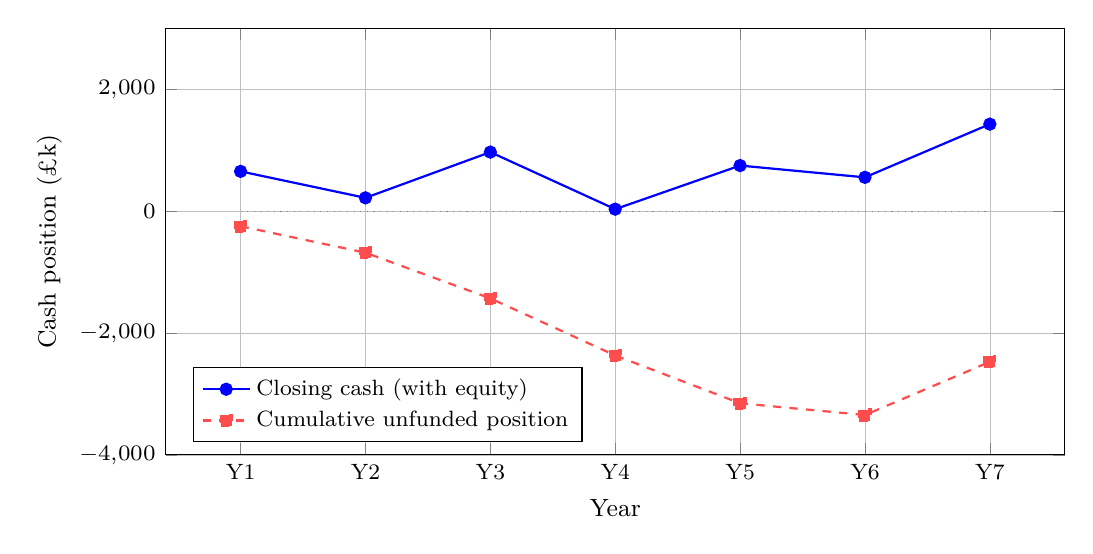
\begin{tikzpicture}
    \begin{axis}[
            width=13cm,
            height=7cm,
            xlabel={Year},
            symbolic x coords={Y1,Y2,Y3,Y4,Y5,Y6,Y7},
            xtick=data,
            grid=major,
            grid style={line width=.1pt, draw=gray!30},
            major grid style={line width=.2pt,draw=gray!50},
            legend style={
                font=\footnotesize,
                at={(0.02,0.98)},
                anchor=north west,
                legend cell align={left},
            },
            tick label style={font=\footnotesize},
            label style={font=\small},
        ylabel={Cash position (\pounds k)},
        ymin=-4000, ymax=3000,
        legend pos=south west,
    ]
    \addplot[thick,blue,mark=*,mark size=2pt] coordinates {(Y1,651.1) (Y2,216.8) (Y3,967.4) (Y4,31.2) (Y5,746.4) (Y6,553.3) (Y7,1426.4)};
    \addplot[thick,red!70,dashed,mark=square*,mark size=2pt] coordinates {(Y1,-248.9) (Y2,-683.2) (Y3,-1432.6) (Y4,-2368.8) (Y5,-3153.6) (Y6,-3346.7) (Y7,-2473.6)};
    \draw[dotted,gray,thin] (axis cs:Y1,0) -- (axis cs:Y7,0);
    \legend{Closing cash (with equity), Cumulative unfunded position}
    \end{axis}
\end{tikzpicture}

\end{document}
